% !TeX spellcheck = es_ES
% Chapter 1

%\chapter{Chapter Title Here} % Main chapter title
%
%\label{Chapter1} % For referencing the chapter elsewhere, use \ref{Chapter1} 

%----------------------------------------------------------------------------------------

% Define some commands to keep the formatting separated from the content 
%\newcommand{\keyword}[1]{\textit{#1}}
%\newcommand{\tabhead}[1]{\textbf{#1}}
%\newcommand{\code}[1]{\texttt{#1}}
%\newcommand{\file}[1]{\texttt{\bfseries#1}}
%\newcommand{\option}[1]{\texttt{\itshape#1}}

%----------------------------------------------------------------------------------------

\chapter{Calibración Eléctrica}
	Con el objetivo de asegurar que la información registrada  por el calorímetro corresponde con un valor específico de potencia, es necesario realizar una calibración eléctrica. Para ello, el equipo cuenta con una resistencia de precisión que envuelve el contenedor de la celda y permite simular, lo mejor posible, la energía liberada en forma de calor cuando una reacción química tiene lugar en la celda. 
	
	Existen dos tipos de calibraciones, la primera es estática, donde la resistencia disipa una potencia conocida, por un tiempo determinado por el usuario, y se espera que la señal registrada por el calorímetro en su estado estacionario coincida con el valor aplicado de potencia. En la calibración dinámica, el sistema aplica 40 \% de la potencia de funcionamiento de la resistencia, registra la pendiente observada y posteriormente incrementa la potencia hasta el 95 \%, a partir de esta información adquiere los par\'ametros de ganancia y cero del equipo.
	\section{Est\'atica}
	\begin{figure}[h]
		\centering
		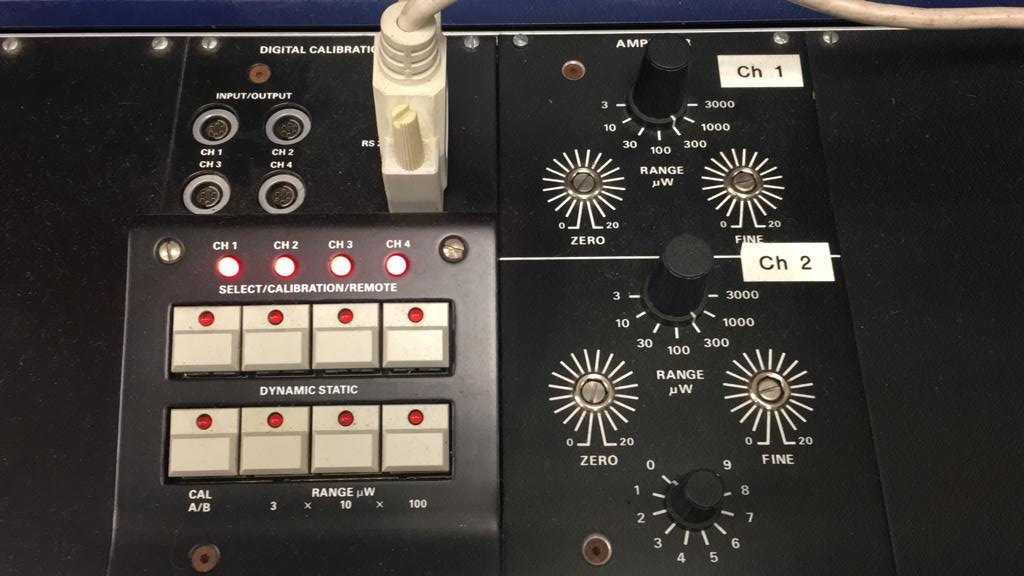
\includegraphics[width=0.7\linewidth]{Figures/controlCal}
		\caption{Control del cero y la ganancia del calor\'imetro}
		\label{fig: controlCal}
	\end{figure}
	
	\section{Din\'amica}


		